\documentclass[]{report}   % list options between brackets
\usepackage{}  % list packages between braces
\usepackage{tikz} % list packages between braces
\usepackage{pgf}  % list packages between braces
\usepackage{graphicx} % list packages between braces
\usepackage{float}
\usepackage{amsmath}
\usepackage{amssymb}
\usepackage{amsfonts}
\usepackage{amsthm}
\usepackage{amsmath}
\usepackage[english]{babel}
\usepackage[a4paper,top=2cm,bottom=2cm,left=3cm,right=3cm,marginparwidth=1.75cm]{geometry}
\usepackage{lipsum}
\usepackage{enumitem, pifont}
\usepackage{xcolor}

% type user-defined commands here

\begin{document}
\hrule
\vspace*{1cm}
\centering
\Large \textbf{ISETB:Professional Master in Advanced Robotics and Artificial Intelligence}
\vspace*{1cm}
\hrule

% Photos and text on the same level
\begin{figure}[h]
    \begin{minipage}[h]{0.2\textwidth}
        \raggedright     % Aligns the photo to the left
        
\includegraphics[width=\textwidth]{logo.jpg}
    \end{minipage}
    \hspace*{0.6\textwidth}
    \begin{minipage}[h]{0.2\textwidth}
        \raggedleft % Aligns the photo to the right
        
\includegraphics[width=\textwidth]{logo_iset.jpg}
    \end{minipage}
\end{figure}
\vspace*{2cm}
% Title text between the lines

\begin{center}
\hrule
\vspace*{1cm}
\Large \textbf {\LARGE PROJET PROPOSAL about USED CARS PRICE PREDICTION APPLICATION}
\vspace*{1cm}
\hrule
\end{center}
\vspace*{2cm}
% Author and date
\begin{center}
  \large Leila Megdiche \& Iheb Mechergui \\
  \today
  \end{center}
  \vspace*{2cm}
\begin{figure}[H]
  \centering
  
\includegraphics[width = 0.4 \linewidth]{Logo_App.jpeg}
  \caption{The Logo Of our Application} \label{exemple-ref-img}
\end{figure}
\vspace*{1cm}
\section{Problems}     % section 1 
\begin{itemize}
  \item [\ding{56}] Lack of transparency:\\
  Buyers and sellers of used cars often struggle with determining the fair market value of a vehicle.
  This lack of transparency can lead to disagreements over pricing and ultimately deter potential buyers and sellers from completing a transaction.
  % Saut de ligne optionnel (aérer)
  
 \item [\ding{56}] Unreliable pricing information:\\
 The price of a used car can vary widely based on factors such as make, model, year, mileage, and condition. 
 Without accurate pricing information, buyers and sellers may not be able to make informed decisions about the value of a car.
 \item [\ding{56}] Limited access to data:\\
 Collecting and analyzing data on used car prices can be time-consuming and challenging.
 Buyers and sellers may not have access to the same data sources, which can lead to disparities in pricing information and ultimately create barriers to completing transactions.\\
  % Saut de ligne (\\) licite pour aérer l
\end{itemize}

\section{The solution: The project Idea}    % section 2
We offer a solution based on our application:
The Used Cars Price Prediction application is a machine learning-based tool designed to help buyers and sellers of used cars make informed pricing decisions.
The application collects data on used car prices and features from various sources, such as online marketplaces and dealerships, and uses this data to predict the fair market value of a vehicle 
based on its make, model, year, mileage, and condition.
\begin{figure}[H]
\centering
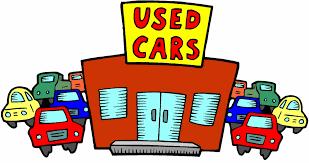
\includegraphics[width = 0.5 \linewidth]{used_cars.jpg}
\caption{Used Cars} \label{exemple-ref-img}
\end{figure}
  

\section{The solution: The project implementation}    % section 3
The project includes several stages, including data collection, preprocessing, feature engineering, model development and evaluation, software interface development, and deployment.
During the data collection stage, a large dataset of used car prices and related features is collected from various sources.
In the preprocessing and feature engineering stage, the data is cleaned and transformed to improve the accuracy of the price prediction model.
Next, various machine learning models, such as linear regression, random forest, and gradient boosting, are trained and evaluated to find the most accurate model for this particular use case. 
\section{Related Papers}     % section 2.1
\subsection{software}
in order to run through this project, we will grasp together all our knowledge to build and test our application inside a JUPYTER NOTEBOOK, we will use PYTHON and JULIA
\subsection{software interface}
we will use VISUAL STUDIO CODE as the envirement of programming where will use 
\begin{itemize}
  \item [\ding{228}] HTML \& CSS \& JAVASCRIPT for the web application.\\ 
  \item [\ding{228}]  LATEX for the report project and the proposal.\\
  \item [\ding{228}]  ANDROID STUDIO for the mobile application.\\
\end{itemize}
  \section{Dataset}         % subsection 2.1.1
  we will use Some of the most popular open-source libraries for machine learning:
\textbf{KAGGLE} and we will import our dataset from this link:  \url {https://www.kaggle.com/datasets/avikasliwal/used-cars-price-prediction}
\end{document}